\documentclass[a4paper,pdftex]{article}

\usepackage{array}
\usepackage{listings}
\usepackage{hopsantut}
\usepackage{framed}

\hypersetup{pdfauthor={Robert Braun and Peter Nordin}, pdftitle={Hopsan Tutorial - Getting Started}, pdfsubject={Hopsan Tutorial}}

\begin{document}
\maketitle{Advanced Usage}

\section*{Introduction}
This tutorial describes more advanced techniques for modeling and simulation with Hopsan. It is recommended to first read the \textit{Getting Started} tutorial, to get a better overview of the program. Start with loading the model file called \texttt{advanced\_usage.hmf}. All following sections assumes this file to be open.

\icon{0}{gfx/Hopsan-Simulate.png}{Load Model File (Ctrl-O)}

\section{System Parameters}
In models with several identical components, it is very impractical to go through all components and change the same parameters in all of them.
Instead, it is desirable to only change the parameters for all components in one place. 
This can be done by using \textit{system parameters}. 
In the example models the piston components are equal.
We want to control the piston areas and the stroke as system parameters.

\begin{tutenumerate}
\tutitem{Open the system parameters widget}
Open the system parameters widget by clicking on the icon in the toolbar:

\icon{0}{gfx/Hopsan-SystemParameter.png}{System Parameters (Ctrl-Shift-Y)}

\tutitem{Add system parameters}
An empty widget appears to the right. Now click on the \textit{Add} button. In the dialog, create the following parameters:

{\renewcommand{\arraystretch}{1.2} 
\begin{tabularx}{0.6\linewidth}{X X X}
\textbf{Name} & \textbf{Value} & \textbf{Type} \\
\specialrule{1.3pt}{0pt}{0pt}
A\_1 & 0.001 & double \\
A\_2 & 0.001 & double \\
s\_l & 1.0 & double
\end{tabularx}
}

\tutitem{Apply system parameters}
Now double-click on the first cylinder to open the \textit{component properties} dialog. To map a parameter to a system parameter, change the value of the parameter to the name of the system parameter. Change the values according to the figure below.

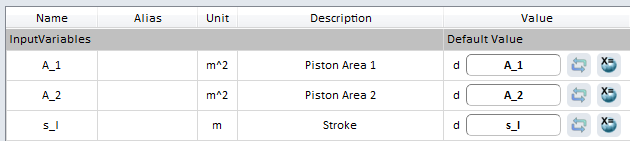
\includegraphics[width=0.8\linewidth]{gfx/advancedusage/systemparameters.png}

It is also possible to choose parameters from a list, by clicking on the globe item to the right of the parameter value. Now do the same thing for the other cylinder. Both cylinders will now use the area and stroke parameters defined in the system parameters widget. If you like to, you can try a few simulations and see that it works as expected.
\end{tutenumerate}

\section{Subsystems}
Large model diagrams can be made simpler and less confusing by moving groups of components to \textit{subsystems}. A subsystem is practically a component consisting of a system of other components. We will now make a subsystems of the two postion servos.

\begin{tutenumerate}
\tutitem{Add a subsystem component}
Locate the \textit{Subsystem} component in the library with the same name and add it to the model:

\vspace{5pt}
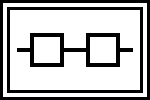
\includegraphics{gfx/advancedusage/subsystem.pdf}

\tutitem{Select and cut components}
Select the valve, piston, mass and tank component from the first position servo. Press Ctrl-X to cut the components.

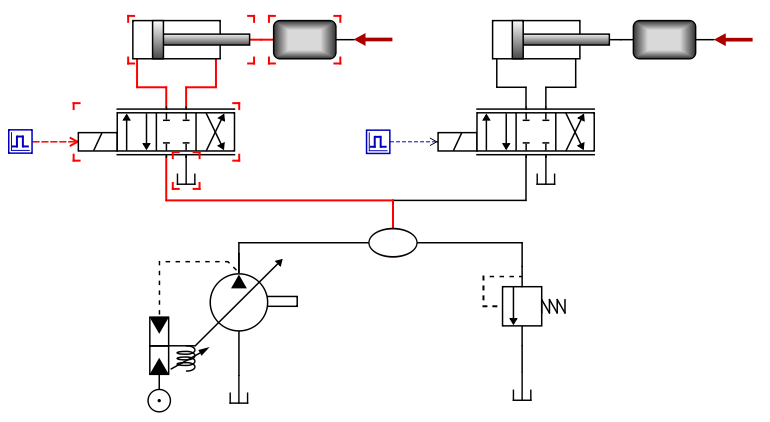
\includegraphics[width=0.85\linewidth]{gfx/advancedusage/componentsforsubsystem.png}

\tutitem{Enter the subsystem and paste components}
Double-click on the subsystem component to enter the system. Paste the cutted components by pressing Ctrl-V.

\tutitem{Add container ports}
Ports in subsystems are defined by \textit{container port} components, located in the Subsystem library folder. Add three container ports to the subsystem, and connect them to the three unconnected ports:

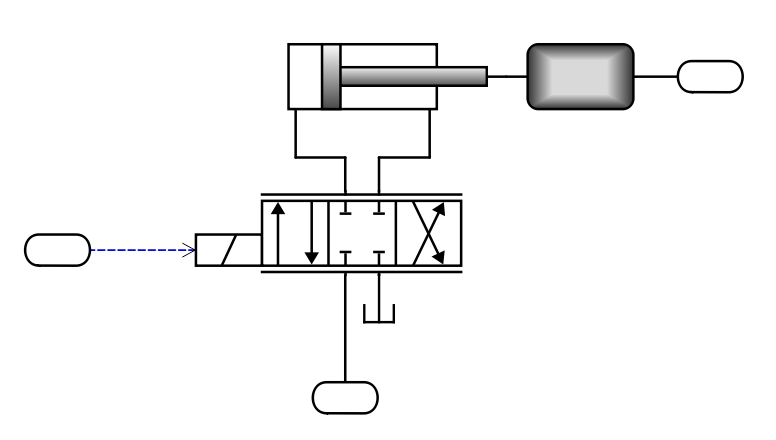
\includegraphics[width=0.6\linewidth]{gfx/advancedusage/systemports.png}

\tutitem{Connect the subsystem to the model}
Return to the top-level system by clicking on the button at the top left corner of the model. The subsystem now has three ports, representing the container ports. Connect them to the model as shown below:

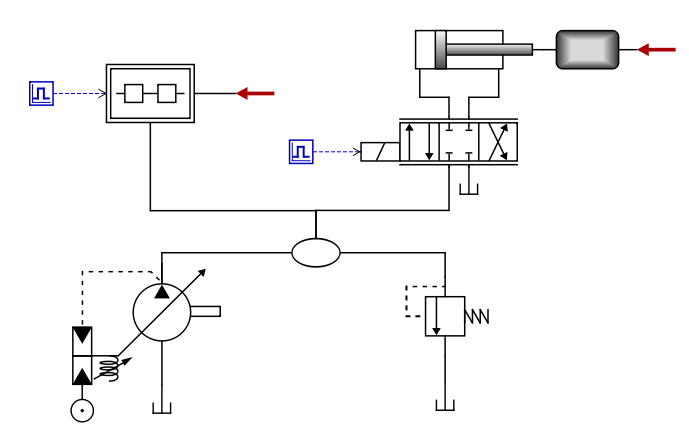
\includegraphics[width=0.85\linewidth]{gfx/advancedusage/connectedsubsystem.png}

\tutitem{Add parameters to subsystem}
Subsystems can have parameters, just like other components. These are created by adding system parameters within the subsystem. Enter the subsystem by double-clicking on it and open the system parameters widget. As you can see, the system parameters from the previous section (A\_1, A\_2 and s\_l) have been added automatically when pasting the components. Now leave the subsystem and return to the top-level system again. Now right-click on the subsystem component and click on \textit{Properties} in the drop-down menu. Go to the \textit{System Parameters} tab. Here we can change the value of the subsystem parameters, which in turn will affect the piston component. System parameters in the top-level system can be propagated down to the subsystem by setting the value of each system parameter to the name of the top-level system parameter, as in the figure below:

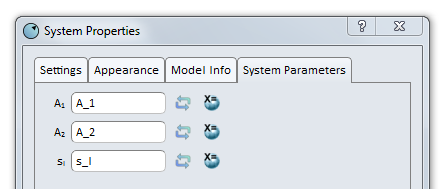
\includegraphics[width=0.6\linewidth]{gfx/advancedusage/subsystemparameters.png}

Everything will now work exactly as before we added the subsystem. If you want to, you can redo the process and create a subsystem for the second postion servo as well.

\end{tutenumerate}

\newpage
\section{Scripting}
Most features in Hopsan can be accessed by writing commands in the terminal widget, located below the workspace. It is also possible to automate repetitive processes by writing script files. 

\begin{tutenumerate}
\tutitem{Getting help}linewidth
Use the \texttt{help} command to display a list of all available commands:

\vspace{5pt}\hspace{10pt}
\begin{minipage}{0.5\linewidth}
\begin{verbatim}
>> help
\end{verbatim}
\end{minipage}
\vspace{5pt}

To show documentation about a specific command, write \texttt{help} followed by the command:

\vspace{5pt}\hspace{10pt}
\begin{minipage}{0.5\linewidth}
\begin{verbatim}
>> help chpa
--------------------------------
 Change parameter value
  Usage: chpa [parameter value]
--------------------------------
\end{verbatim}
\end{minipage}
\vspace{5pt}

\tutitem{Changing parameters}
To change a parameters in the current model, you can use the \texttt{chpa} (\underline{ch}ange \underline{pa}rameters) command. Try to change the oil density parameter in the first valve component. The component is called "Valve1", the parameter name is "rho" and the variable is called "y". The full name of the parameter is thus "Valve1.rho.y".

\vspace{5pt}\hspace{10pt}
\begin{minipage}{0.5\linewidth}
\begin{verbatim}
>> chpa Valve1.rho.y 900
Changed value for 1 parameters.
\end{verbatim}
\end{minipage}
\vspace{5pt}

In many cases it is necessary to change several parameters at the same time. The oil density, for example, should obviously be the same in both valve components. This can be done by using \textit{wildcards}, represented by the asterisk (*) symbol. Writing "*x" or example will modify all parameters that ends with an "x". "*x*y" will modify all parameters that contains the letter "x" and ends with the letter "y". Now change all parameters named "rho" by writing:

\vspace{5pt}\hspace{10pt}
\begin{minipage}{0.5\linewidth}
\begin{verbatim}
>> chpa *.rho.y 900
Changed value for 2 parameters.
\end{verbatim}
\end{minipage}
\vspace{5pt}

\tutitem{Run a simulation}
Once all parameters have been set, the simulation can be started by the "sim" command. Try this now!

\vspace{5pt}\hspace{10pt}
\begin{minipage}{0.5\linewidth}
\begin{verbatim}
>> sim
[09:44:42] Info: In advanced_usage;  Using single-threaded algorithm.
[09:44:42] Info: Simulated 'advanced_usage' successfully! Initialization time: 4 ms, Simulation time: 21 ms
\end{verbatim}
\end{minipage}
\vspace{5pt}

\tutitem{Plot results}
When the simulation is finished, variables can be plotted with the "chpv" (\underline{ch}ange \underline{p}lot \underline{v}ariable) command. Now plot the system pressure. This can for example be found as the variable "p" in port "P2" in the component named "Pump". The full variable name is thus "Pump.P2.p".

\vspace{5pt}\hspace{10pt}
\begin{minipage}{0.5\linewidth}
\begin{verbatim}
>> chpv Pump.P2.p
\end{verbatim}
\end{minipage}
\vspace{5pt}

\tutitem{Writing a script file}
Script files are useful for running several commands at the same time, and for reusing code. It is also possible to use loops (such as "while") and conditional statements, like "if". We will now create a script file and call it. First, check the present working directory of Hopsan with the "pwd" command:

\vspace{5pt}\hspace{10pt}
\begin{minipage}{0.5\linewidth}
\begin{verbatim}
>> pwd
C:/Users/Username/Documents/Hopsan
\end{verbatim}
\end{minipage}
\vspace{5pt}

It is possible to list the files in the folder with the "ls" command, and change directory with the "cd" command. Now change to the "Scripts" directory.

\vspace{5pt}\hspace{10pt}
\begin{minipage}{0.5\linewidth}
\begin{verbatim}
>> ls
.
..
Backup
Libraries
LogData
Models
Scripts
\end{verbatim}
\end{minipage}
\vspace{5pt}

\vspace{5pt}\hspace{10pt}
\begin{minipage}{0.5\linewidth}
\begin{verbatim}
>> cd Scripts
C:/Users/Username/Documents/Hopsan/Scripts
\end{verbatim}
\end{minipage}
\vspace{5pt}

Now use an external editor, for example Notepad in Windows, to create a script file in this folder. We want to create a file that simulates the system five times with five different levels of system pressure, and then plots all five results in one diagram. Write the following code, and save the file as "tutorial.hcom".

\vspace{5pt}
\texttt{\textbf{tutorial.hcom}}
\vspace{3pt}\\
\hspace{10pt}
\begin{minipage}{0.4\linewidth}
\begin{framed}
\begin{verbatim}
rmvar Pump.P2.p@*
pref.p.y=1e7
i=0
while(i<5)
  sim
  pref.p.y=pref.p.y+2e6
  i=i+1
repeat
chpv Pump.P2.p@*
\end{verbatim}%
\vspace{-10pt}
\end{framed}
\end{minipage}
\vspace{5pt}

The first command removes all previous generations of the pump pressure variable. The last two characters ("\texttt{@*}") means "at all generations". Then we set the reference pressure parameter to 100 bar (1e7 Pa). We then loop five steps, and for each step we simulate the model and then increase the pressure with 20 bar (2e6 Pa). We thus simulate the system for 100, 120, 140, 160 and 180 bar. After the loop we plot all generations of the system pressure. Now launch the script by the "exec" command!

\vspace{5pt}\hspace{10pt}
\begin{minipage}{0.5\linewidth}
\begin{verbatim}
>> exec tutorial.hcom
\end{verbatim}
\end{minipage}
\vspace{5pt}

If all goes well, the model shall be simulated five times and then a plot window with five curves will appear.
\end{tutenumerate}

%
%\section{Importing Data}
%- Importera en körcykel för en av cylindrarna från en CSV-fil
%- Importera även filen som variabel
%
%\section{Exporting Data}
%- Beskriv hur man exporterar från plottfönstret
%- Beskriv hur man exporterar från HCOM

\end{document}